%=============================================================================
%  CHAPTER 3 — SPRINT 0: ARCHITECTURE AND GENERAL CONCEPTION
%=============================================================================
\chapter{Sprint 0: Architecture and General Conception}

\clearpage
\section*{Introduction}

In a Scrum project, Sprint 0 does not yet deliver a usable feature. Its role is to put in place everything the team will need before the first functional sprint can be planned: the technical architecture, the shared vocabulary, the general data model, and the recurring conventions that the rest of the iterations will reuse. We treated Sprint 0 of ForsaDrive in the same spirit. Over roughly the first two weeks of the internship, the focus was less on producing screens and more on settling the questions that, if left open, would have slowed down every later sprint. This chapter reports on that work. It describes the architecture that was retained for the platform, the way the most representative use cases of the global diagram were refined, and the structural backbone of the application through its class diagram and its relational schema.

\section{Sprint 0 Backlog and Objectives}

Before describing the deliverables, it is useful to recall the perimeter of Sprint~0. The product backlog at this point did not contain user stories in the strict sense, since no end user feature was yet targeted. It contained the technical and methodological items that the team needed to validate before starting Sprint~1. Table~\ref{tab:sprint0_backlog} gives an extract of what was placed in this preliminary backlog.

\begin{table}[H]
\centering
\caption{Sprint 0 backlog — preparatory items}
\label{tab:sprint0_backlog}
\begin{tabular}{|p{3.5cm}|p{9cm}|c|}
\hline
\textbf{Item} & \textbf{Description} & \textbf{Estimate (h)} \\
\hline
Architecture choice & Decide on the deployment topology, the API style, and the boundary with external services. & 6 \\
\hline
Stack validation & Confirm that PHP, SQLite, and Flutter can share the same database file in WAL mode. & 8 \\
\hline
Repository layout & Set up the monorepo with the \texttt{web/}, \texttt{mobile/}, and shared backend folders. & 4 \\
\hline
Use case refinement & Detail the four most sensitive use cases identified in chapter~2. & 10 \\
\hline
Class diagram & Produce the structural model covering the core and the secondary entities. & 12 \\
\hline
Relational schema & Translate the class diagram into a normalized schema, with constraints and indexes. & 8 \\
\hline
Coding conventions & Agree on naming, error format, and commit message style. & 3 \\
\hline
\end{tabular}
\end{table}

The estimates are deliberately rough. As is often the case during Sprint~0, several items overlapped: the architecture choice and the stack validation, for example, could not be separated cleanly because validating the stack \textit{was} part of choosing the architecture. The team kept track of the work through a simple Trello board with three columns and updated it at the end of each working day.

\section{General Architecture}

\subsection{Client--Server Topology}

ForsaDrive is organized around a classic client--server topology. A unified REST API is exposed by a backend server and is consumed by two distinct clients: a web application targeted at administrators and at desktop users, and a mobile application that covers the daily usage of drivers and passengers. This separation has two main benefits. It allows the two interfaces to evolve at their own pace, as long as the API contract remains stable, and it avoids duplicating the business logic on the client side, where it would be both harder to maintain and easier to bypass. External services such as the payment gateway, the notification service, and the file storage that hosts student identity documents are reached exclusively through the backend, so that no sensitive credential is ever exposed on a client device.

\begin{figure}[H]
    \centering
    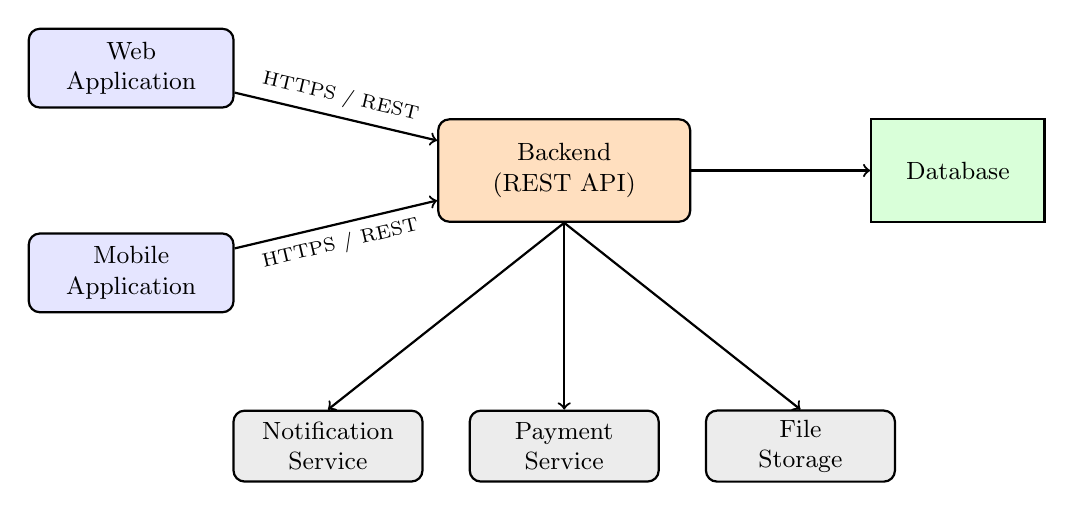
\begin{tikzpicture}[
        every node/.style={font=\small},
        client/.style={draw, rounded corners, minimum width=2.6cm, minimum height=1cm, fill=blue!10, thick, align=center},
        server/.style={draw, rounded corners, minimum width=3.2cm, minimum height=1.3cm, fill=orange!25, thick, align=center},
        db/.style={draw, minimum width=2.2cm, minimum height=1.3cm, fill=green!15, thick, align=center},
        ext/.style={draw, rounded corners, minimum width=2.4cm, minimum height=0.9cm, fill=gray!15, thick, align=center}
    ]
        \node[client] (web)    at (0,  1.3) {Web\\ Application};
        \node[client] (mobile) at (0, -1.3) {Mobile\\ Application};
        \node[server] (api) at (5.5, 0) {Backend\\ (REST API)};
        \node[db] (db) at (10.5, 0) {Database};
        \node[ext] (notif) at (2.5, -3.5) {Notification\\ Service};
        \node[ext] (pay)   at (5.5, -3.5) {Payment\\ Service};
        \node[ext] (store) at (8.5, -3.5) {File\\ Storage};
        \draw[->, thick] (web)        -- (api) node[midway, above, sloped] {\scriptsize HTTPS / REST};
        \draw[->, thick] (mobile)     -- (api) node[midway, below, sloped] {\scriptsize HTTPS / REST};
        \draw[->, thick] (api)        -- (db);
        \draw[->, thick] (api.south)  -- (notif.north);
        \draw[->, thick] (api.south)  -- (pay.north);
        \draw[->, thick] (api.south)  -- (store.north);
    \end{tikzpicture}
    \caption{Client--server architecture of ForsaDrive}
    \label{fig:client_server_architecture}
\end{figure}

\subsection{Three-Tier Internal Organization}

Internally, the backend follows a three-tier organization that separates presentation, business logic, and data persistence. This decomposition reflects a deliberate effort to isolate the parts of the system that change at different rhythms: the presentation tier evolves with the user interface, the application tier with the business rules, and the data tier with the persistence model.

\begin{description}[noitemsep]
    \item[Presentation tier.] Composed of the web and mobile applications, this layer is responsible for user interaction, form validation on the client side, and rendering. It never accesses the database directly and only communicates with the application tier through the REST API.
    \item[Application tier.] Contains the business rules of ForsaDrive: route publication, booking logic, prepayment computation, application of the student discount, ride lifecycle, ratings and reliability scoring, and complaint handling. It is exposed through a REST API secured by bearer tokens.
    \item[Data tier.] Stores persistent information such as users, routes, bookings, payments, ratings, and messages. It is accessed exclusively through the application tier, which guarantees the integrity of the business rules at all times.
\end{description}

\begin{figure}[H]
    \centering
    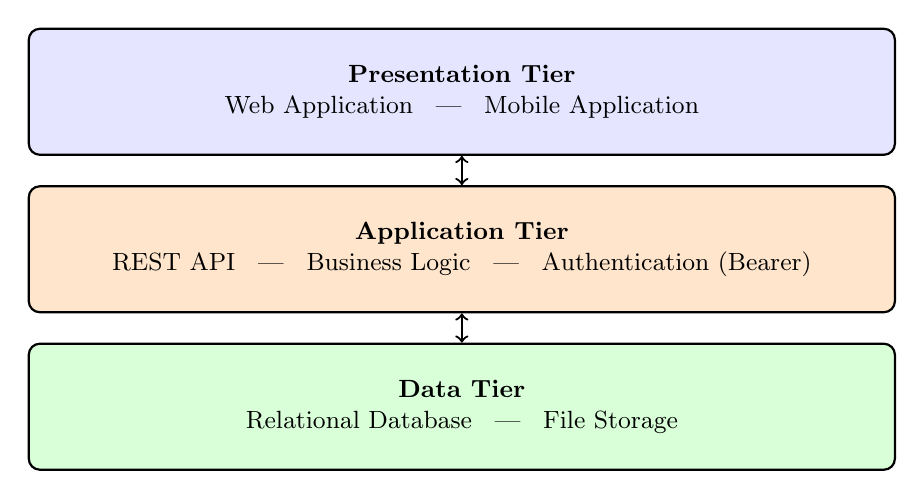
\begin{tikzpicture}[
        every node/.style={font=\small, align=center},
        tier/.style={draw, rounded corners, minimum width=11cm, minimum height=1.6cm, thick}
    ]
        \node[tier, fill=blue!10]   (pres) at (0, 4) {\textbf{Presentation Tier}\\ Web Application \;\;|\;\; Mobile Application};
        \node[tier, fill=orange!20] (app)  at (0, 2) {\textbf{Application Tier}\\ REST API \;\;|\;\; Business Logic \;\;|\;\; Authentication (Bearer)};
        \node[tier, fill=green!15]  (data) at (0, 0) {\textbf{Data Tier}\\ Relational Database \;\;|\;\; File Storage};
        \draw[<->, thick] (pres) -- (app);
        \draw[<->, thick] (app)  -- (data);
    \end{tikzpicture}
    \caption{Three-tier organization of the platform}
    \label{fig:three_tier_architecture}
\end{figure}

\subsection{External Services}

In addition to its own three tiers, the backend interacts with three external building blocks. The \textbf{payment service} is responsible for the fifty-percent prepayment that confirms a booking. In the first version of ForsaDrive this service is simulated through a local wallet, since no Tunisian payment gateway could be integrated within the duration of the internship; the architecture, however, is designed so that this layer can be replaced by a real provider such as Konnect or Paymee without changing the booking logic itself. The \textbf{notification service} delivers booking, payment, and message alerts to drivers and passengers, both through push notifications on the mobile application and through email when relevant. Finally, a dedicated \textbf{file storage} keeps student identity documents and profile pictures separately from the relational database, which keeps the SQLite file small and allows documents to be served through short-lived signed URLs that protect them from unauthorized access.

\subsection{Security Mechanisms}

Authentication relies on randomly generated bearer tokens delivered after a successful login. Every protected endpoint validates the token, extracts the user identity from the \texttt{api\_tokens} table, and checks the associated role before executing the requested operation. Passwords are hashed with \texttt{password\_hash} (bcrypt) and are never stored or transmitted in clear. All communications go through HTTPS in production, and sensitive operations such as payment, account suspension, or student verification are logged on the server side for audit purposes. Identity documents stored in the file service are accessible only to authenticated administrators, through signed URLs that expire after a short delay. Together these mechanisms reduce the attack surface of the platform and align its handling of personal data with the expectations of users entrusting their identity documents to the system.

\section{Refinement of the Main Use Cases}

The global use case diagram of ForsaDrive, already presented in chapter~2, regroups the functionalities of the platform around four actors -- the \textit{Passenger}, the \textit{Driver}, the \textit{Admin}, and the \textit{System}. The latter is responsible for automated operations such as discount calculation, reliability scoring, and notification dispatching. Each actor is restricted to a coherent set of use cases, and a few of them are connected through \texttt{<<include>>} or \texttt{<<extend>>} relationships when an operation must trigger an automated step or when a behavior is optional.

The textual refinement of the four most representative use cases is given below. These four were selected because they cut across the largest number of components and therefore drove the deepest design decisions of the project. The remaining use cases follow a similar pattern and are described, sprint by sprint, in chapters~4 and~5.

\subsection{Use Case: Publish a Route}

\textbf{Actor:} Driver.\\
\textbf{Precondition:} The driver is authenticated, the account is active, and a vehicle has been registered on the profile.\\
\textbf{Main scenario:}
\begin{enumerate}[noitemsep]
    \item The driver selects the action of creating a new route.
    \item The system displays the route creation form.
    \item The driver fills in the origin, the destination, the departure date and time, the price per seat, and the number of available seats.
    \item The driver confirms the creation.
    \item The system validates the data, persists the route with the status \textit{ACTIVE}, and notifies the passengers whose saved searches match the new offer.
\end{enumerate}
\textbf{Alternative scenarios:}
\begin{itemize}[noitemsep]
    \item If a mandatory field is missing or invalid, the system displays an error message and the route is not created.
    \item If the driver account is suspended, the system rejects the request with an explanatory message.
    \item If no vehicle is registered yet, the driver is redirected to the vehicle registration page.
\end{itemize}

\subsection{Use Case: Book a Ride}

\textbf{Actor:} Passenger.\\
\textbf{Precondition:} The passenger is authenticated and at least one seat is available on the selected route.\\
\textbf{Main scenario:}
\begin{enumerate}[noitemsep]
    \item The passenger searches for routes by entering origin, destination, and date.
    \item The system returns the matching routes and applies the student discount on the displayed price if the passenger is a verified student.
    \item The passenger opens the details of a route and selects the number of seats.
    \item The system computes the total amount and the fifty-percent prepayment.
    \item The passenger confirms the booking and the prepayment.
    \item The system processes the prepayment, registers the booking with the status \textit{PENDING}, and notifies the driver.
\end{enumerate}
\textbf{Alternative scenarios:}
\begin{itemize}[noitemsep]
    \item If the prepayment fails, the booking is not created and the passenger is invited to retry or to cancel.
    \item If the seat becomes unavailable between the selection and the confirmation, the booking is rejected and the passenger is informed.
    \item If the driver later refuses the booking, the prepayment is automatically refunded.
\end{itemize}

\subsection{Use Case: Verify Student Status via Email OTP}

\textbf{Actor:} Passenger (Student).\\
\textbf{Precondition:} The passenger is authenticated and possesses a valid university email address whose domain is listed in the platform's recognized domain table.\\
\textbf{Main scenario:}
\begin{enumerate}[noitemsep]
    \item The passenger navigates to the student verification screen and enters a university email address.
    \item The system checks the email domain against the \textit{student\_domains} table maintained by the administrator.
    \item If the domain is recognized, the system generates a six-digit OTP, stores it with a ten-minute expiry, and dispatches it by email to the provided address.
    \item The passenger enters the received code on the verification screen.
    \item The system validates the code, marks the account as \textit{is\_student = true}, and records the verification event in the audit log.
    \item The fifty-percent student discount is automatically applied to all future bookings from this account.
\end{enumerate}
\textbf{Alternative scenarios:}
\begin{itemize}[noitemsep]
    \item If the domain is not in the recognized list, the system rejects the request and shows the list of accepted university domains.
    \item If the code has expired, the student is invited to request a new one.
    \item After five consecutive incorrect attempts the current code is invalidated and the student must request a new one.
\end{itemize}

\subsection{Use Case: Driver Application and Admin Approval}

\textbf{Actors:} Passenger (applicant) and Administrator.\\
\textbf{Precondition:} The applicant is authenticated as a passenger.\\
\textbf{Main scenario:}
\begin{enumerate}[noitemsep]
    \item The applicant opens the \textit{Become a Driver} form and fills in personal details, license number, and vehicle information.
    \item The system stores the application with the status \textit{PENDING} and notifies the administrator.
    \item The administrator reviews the application in the dedicated tab of the admin panel.
    \item Upon approval, the system creates the driver profile, the vehicle record, switches the user role to \textit{DRIVER}, and notifies the applicant.
\end{enumerate}
\textbf{Alternative scenario:}
\begin{itemize}[noitemsep]
    \item Upon rejection, the system stores the rejection reason on the application and notifies the applicant. The user remains a passenger.
\end{itemize}

\section{Class Diagram}

The class diagram describes the structural backbone of the application. Given the breadth of the platform, the diagram regroups around twenty classes that cover not only the core booking entities but also the secondary features that have been identified as relevant for a Tunisian carpooling platform: student verification, complaints, ratings, route boosting, social feed, and analytics. The full diagram is shown in Figure~\ref{fig:class_diagram}.

\begin{figure}[H]
    \centering
    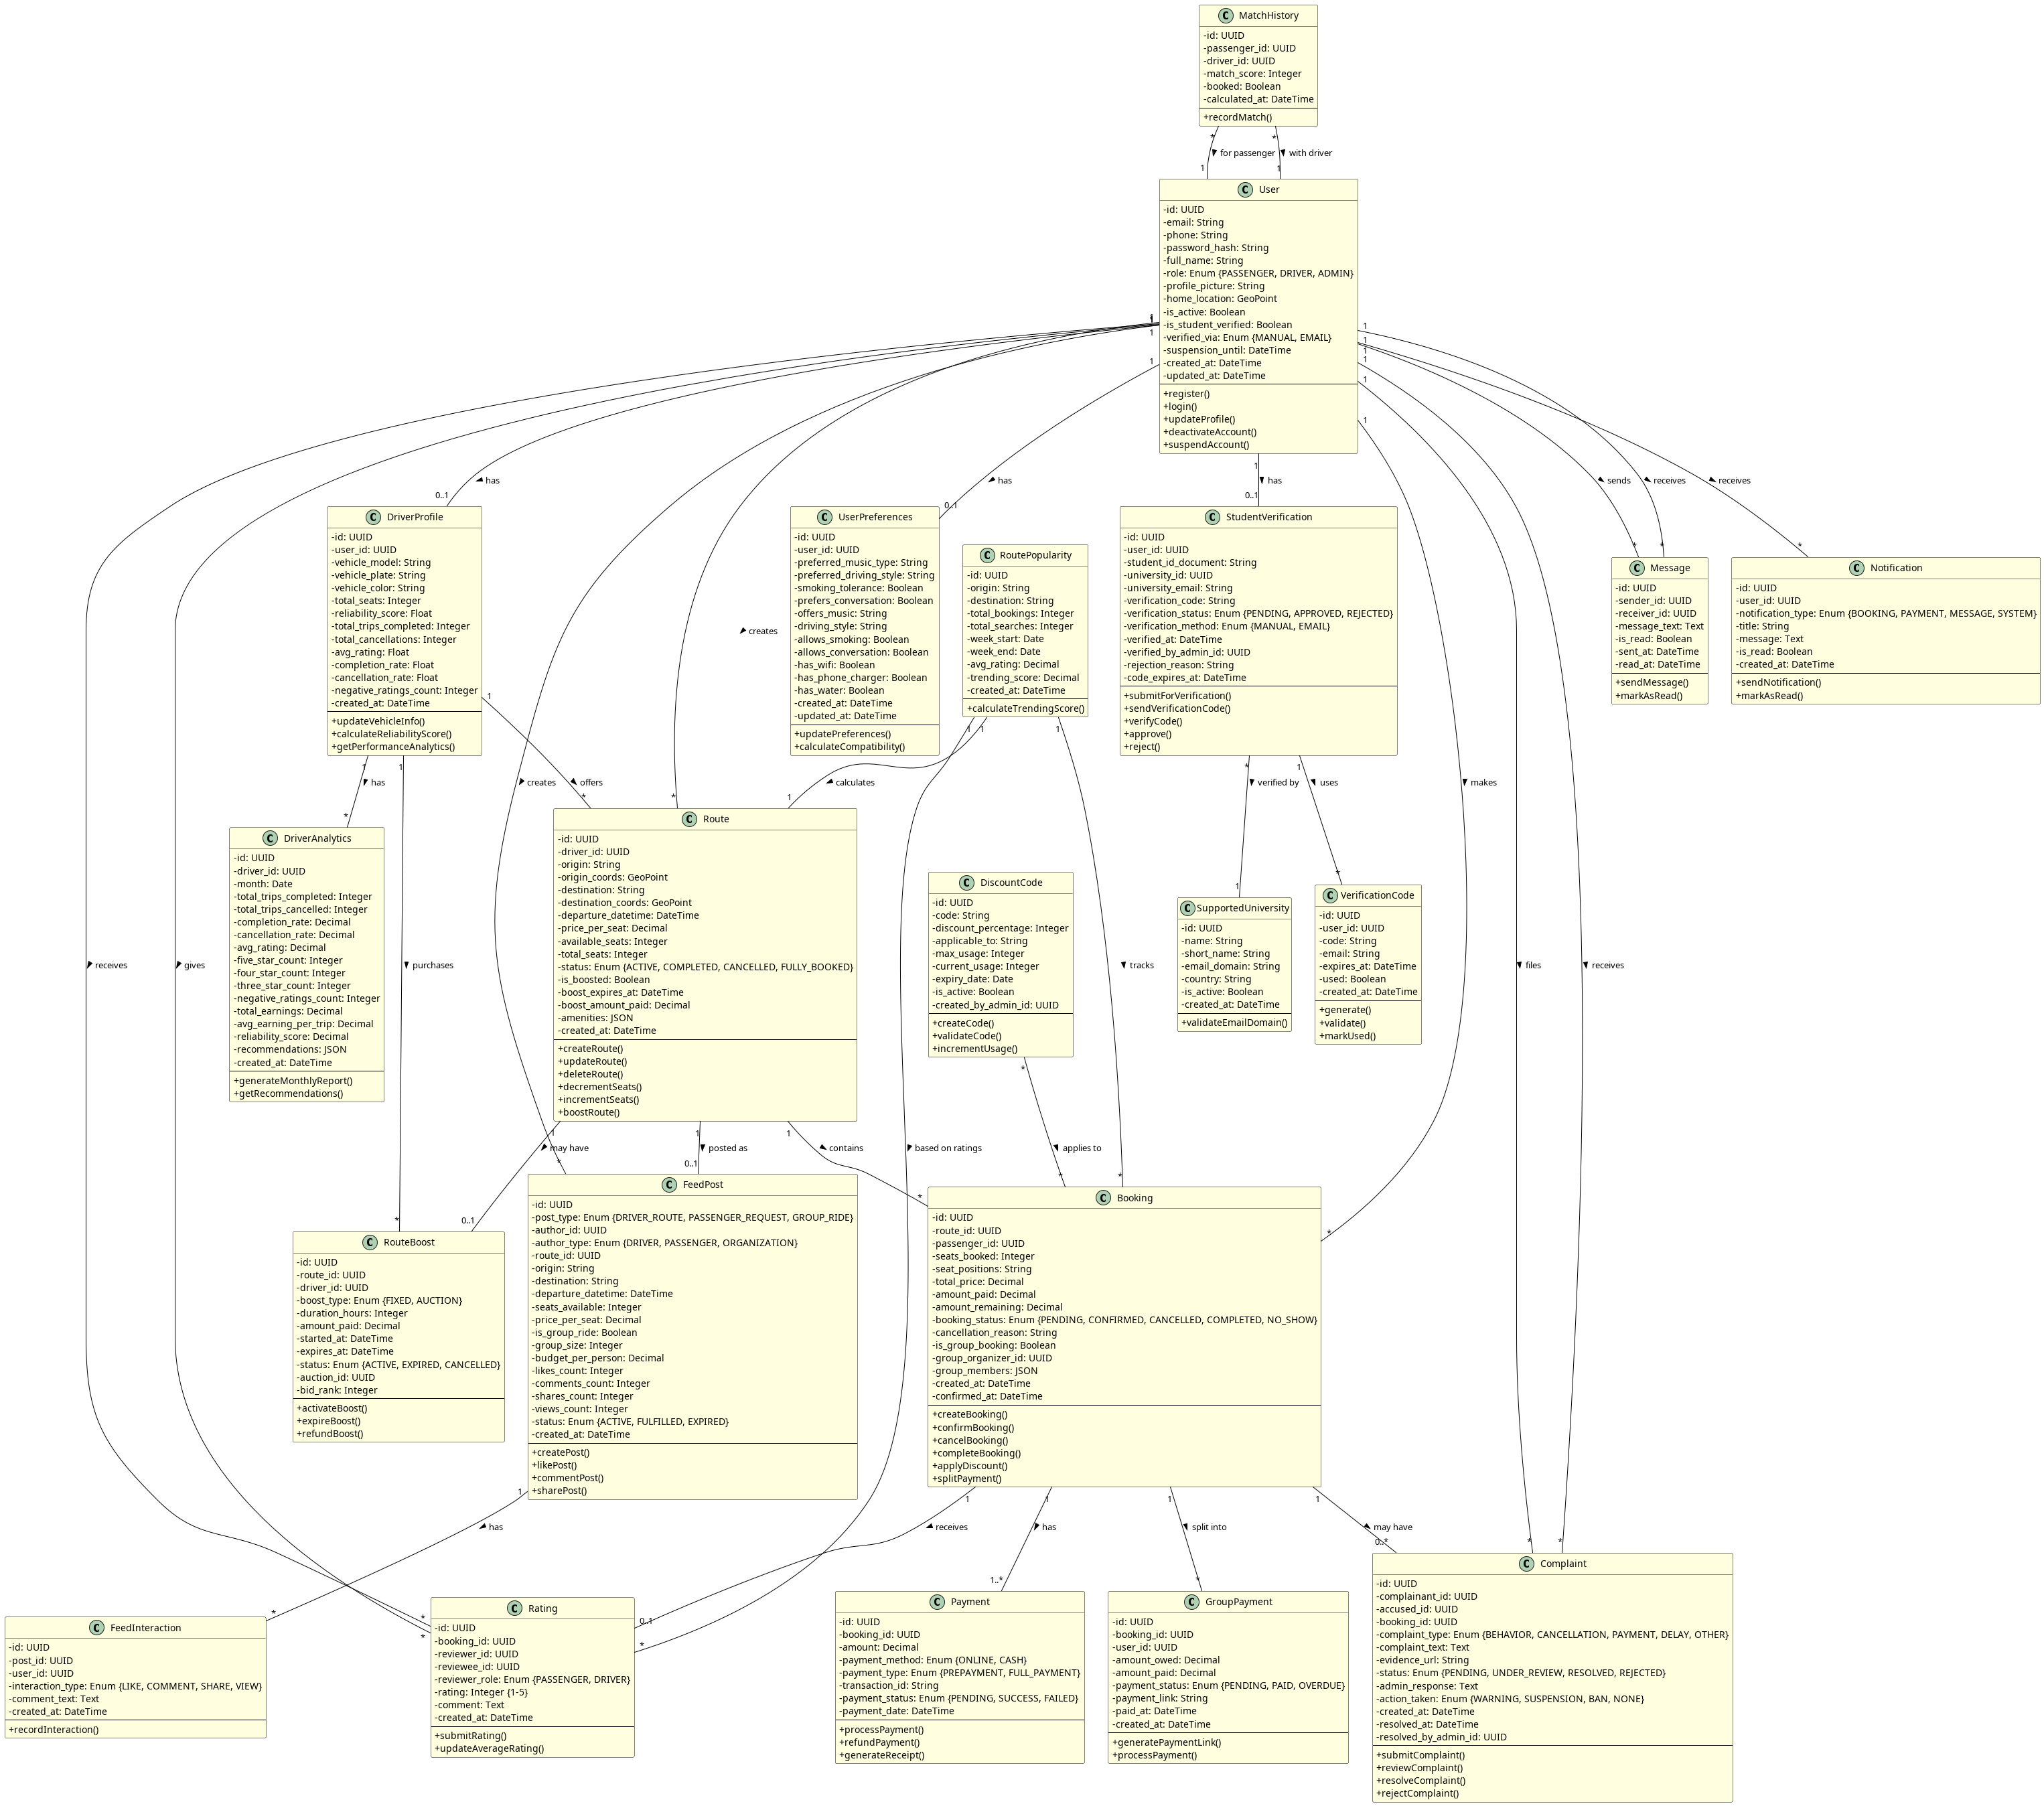
\includegraphics[width=\textwidth, height=0.9\textheight, keepaspectratio]{forsadrive_class_diagram.png}
    \caption{Class diagram of ForsaDrive}
    \label{fig:class_diagram}
\end{figure}

For readability, the main classes are organized into five logical groups.

\paragraph{Users and profiles.} The class \textit{User} represents any registered account and centralizes the credentials, the personal information, the verification status, and the role (\textit{PASSENGER}, \textit{DRIVER}, or \textit{ADMIN}). It is enriched by \textit{DriverProfile}, which holds the vehicle information and the reliability indicators of a driver, and by \textit{UserPreferences}, which describes the preferred travel conditions of a user (music, conversation, smoking tolerance, on-board amenities).

\paragraph{Trips and bookings.} The class \textit{Route} represents a ride offered by a driver, with its origin, its destination, its date, its price, and its available seats. \textit{Booking} represents a reservation made by a passenger on a route and stores the booked seats, the total amount, the prepayment, and the booking status. The optional class \textit{GroupPayment} models the splitting of a booking among several passengers traveling together.

\paragraph{Payments and ratings.} The class \textit{Payment} represents the financial operations linked to a booking, whether it is the prepayment or the final settlement. \textit{Rating} represents the feedback left by a user after a completed trip and feeds back into the average score and the reliability indicators stored on \textit{DriverProfile}.

\paragraph{Verification and discounts.} The class \textit{StudentVerification} stores a verification request, with the uploaded document, the declared university, and the decision of the administrator. It is supported by \textit{SupportedUniversity}, which lists the institutions whose email domains are recognized by the platform, and by \textit{VerificationCode}, which manages email verification codes. The class \textit{DiscountCode} models promotional codes that can be applied at booking time.

\paragraph{Communication and moderation.} The classes \textit{Message} and \textit{Notification} carry the conversations between users and the alerts emitted by the system. \textit{Complaint} allows a user to report a problem after a trip and gives the administrator the means to take action, ranging from a warning to a permanent ban.

Around these core classes, complementary entities such as \textit{DriverAnalytics}, \textit{RoutePopularity}, \textit{MatchHistory}, \textit{RouteBoost}, \textit{FeedPost}, and \textit{FeedInteraction} support the analytical and social dimension of the platform without polluting the central booking workflow.

\section{Database Design}

The class diagram has been translated into a relational model that serves as the schema of the backend database. The translation follows the standard rules: each persistent class becomes a table, each one-to-many association becomes a foreign key, and many-to-many associations are realized through dedicated join tables.

\subsection{Logical Schema}

The logical schema below uses the conventional notation, where primary keys are underlined and foreign keys are marked with the \# symbol. For the sake of readability, only the most representative tables are listed.

\begin{itemize}[noitemsep]
    \item \textbf{User} (\underline{id\_user}, full\_name, email, phone, password\_hash, role, profile\_picture, is\_active, is\_student\_verified, created\_at, updated\_at)
    \item \textbf{DriverProfile} (\underline{id\_driver\_profile}, \#id\_user, vehicle\_model, vehicle\_plate, vehicle\_color, total\_seats, avg\_rating, reliability\_score, completion\_rate, cancellation\_rate, created\_at)
    \item \textbf{UserPreferences} (\underline{id\_preferences}, \#id\_user, preferred\_music\_type, prefers\_conversation, smoking\_tolerance, has\_wifi, has\_phone\_charger)
    \item \textbf{Route} (\underline{id\_route}, \#id\_driver, origin, destination, departure\_datetime, price\_per\_seat, total\_seats, available\_seats, status, is\_boosted, created\_at)
    \item \textbf{Booking} (\underline{id\_booking}, \#id\_route, \#id\_passenger, seats\_booked, seat\_positions, total\_price, amount\_paid, amount\_remaining, booking\_status, created\_at, confirmed\_at)
    \item \textbf{Payment} (\underline{id\_payment}, \#id\_booking, amount, payment\_method, payment\_type, transaction\_id, payment\_status, payment\_date)
    \item \textbf{Rating} (\underline{id\_rating}, \#id\_booking, \#id\_reviewer, reviewer\_role, score, comment, created\_at)
    \item \textbf{StudentVerification} (\underline{id\_verification}, \#id\_user, \#id\_university, student\_id\_document, university\_email, verification\_status, verified\_at, \#id\_admin, rejection\_reason)
    \item \textbf{SupportedUniversity} (\underline{id\_university}, name, short\_name, email\_domain, country, is\_active)
    \item \textbf{DiscountCode} (\underline{id\_discount}, code, discount\_percentage, applicable\_to, max\_usage, current\_usage, expiry\_date, is\_active, \#id\_admin)
    \item \textbf{Message} (\underline{id\_message}, \#id\_sender, \#id\_receiver, message\_text, is\_read, sent\_at, read\_at)
    \item \textbf{Notification} (\underline{id\_notification}, \#id\_user, notification\_type, title, message, is\_read, created\_at)
    \item \textbf{Complaint} (\underline{id\_complaint}, \#id\_complainant, \#id\_accused, \#id\_booking, complaint\_type, complaint\_text, evidence\_url, status, action\_taken, created\_at, resolved\_at, \#id\_admin)
\end{itemize}

\subsection{Constraints and Indexing}

A few business rules deserve to be enforced at the database level rather than only in the application code, since this guarantees their consistency even when the data is touched outside the normal application paths. The number of available seats on a route is constrained between zero and the total number of seats. The booking status follows a controlled state machine (\textit{PENDING}, \textit{CONFIRMED}, \textit{CANCELLED}, \textit{COMPLETED}, \textit{NO\_SHOW}) and the corresponding transitions are checked before any update. Indexes are added on the columns that are frequently used for filtering, in particular the origin and the destination of a route, the departure date, and the foreign keys that link bookings to their route and to their passenger. These indexes ensure that the search operation, which is the most frequent action on the platform, remains responsive even as the volume of data grows.

\section{Sprint 0 Review}

At the end of Sprint~0 the team held a review with the supervising engineer. The architectural choices were validated, with one notable adjustment: the initial intention to use a separate authentication library was abandoned in favor of a lighter, in-house token mechanism stored in an \texttt{api\_tokens} table. This kept the backend free of external dependencies that the team did not feel confident maintaining within the available time. The class diagram was approved with minor renaming, and the database schema was retained in its first version. The repository layout, the conventions, and the use case refinements were also accepted. With these foundations in place, the team could enter Sprint~1 with a clear backlog and a stable structure to build on.

\section*{Conclusion}

This chapter described the work of Sprint~0, whose role was to prepare the ground for the functional sprints that follow. The general architecture clarified the boundary between the clients, the backend, and the external services, and identified the security mechanisms that protect the platform. The four most representative use cases were refined in textual form to expose their internal logic and the alternative scenarios. Finally the class diagram and the relational schema laid down the data foundations that every subsequent sprint will reuse. The next chapter opens the first release of the product and reports on Sprint~1 and Sprint~2, which together deliver the foundational features and the core ride-and-booking workflow.
